
Aquest projecte consisteix en dissenyar una aplicació per a la gestió automatitzada d'un pàrquing inte\l.ligent.
Aquest control es basa en l'entrada i sortida de vehicles d'aquest pàrquing fent servir altres alternatives
al lector de matrícules convencional. A més a més, l'aplicació tindrà un registre de l'estança de cada usuari,
com també la part de configuració pels treballadors.

Algunes d'aquestes alternatives són la comunicació Bluetooth i els codis QR.
En aquest projecte se centra a crear una aplicació on s'utilitza els codis QR.

També, aquesta aplicació dóna l'eina perquè l'usuari faci els pagaments a través d'ella d'una manera segura.

\section{Objectius}

L'objectiu es pot dividir en els punts següents:

\begin{itemize}
    \item Buscar informació sobre els generadors i lectors dels codis QR, com també dels lectors de matrícules i la comunicació Bluetooth.
    \item Aprendre a dissenyar un \emph{backend} i un \emph{frontend}.
    \item Aprendre tots els passos que comporta la creació d'una aplicació i fer-los segons les necessitats del projecte.
    \item Dissenyar un sistema on emmagatzemar les dades, una base de dades. Aprendre MySQL.
    \item Dissenyar l'aplicació perquè l'usuari tingui un bon aprenentatge quan entri per a primer cop, aquesta tingui una eficiència excepcional i sobretot hi hagi seguretat.
    \item Triar dues framework per al desenvolupament de l'aplicació, una per el \emph{backend} i l'altre per el \emph{frontend}.
    \item Aprendre els passos de la framework de React, com també la del Laravel.
\end{itemize}

\section{Conceptes previs}

\begin{itemize}
    \item El \emph{back-end} és la capa d'accés a les dades, és la lògica que fa que una pàgina web funcioni,
    cosa que queda amagada als ulls de l'usuari. Determina que tan bé s'executarà l'aplicació i quina
    experiència obtindrà l'usuari del seu ús, positiva o negativa.
    Es fan servir habitualment llenguatges com PHP, Javascript, Python i Ruby, entre d'altres.
    \item El \emph{front-end} és la part del desenvolupament que es dedica el disseny,
    des de l'estructura del lloc fins als estils com colors, fons, mides fins a arribar a les animacions i efectes.
    És aquesta part de la pàgina amb què interaccionen els usuaris, és tot el que el visitant veu i experimenta
    de manera directa.
    \item \emph{MySQL} és un sistema de gestió de bases de dades relacional que usa el llenguatge SQL per comunicar-s'hi. Algunes
    d'aquestes comunicacions poden ser consultar les dades, manipular-les, etc.
    \item Una \emph{framework} és una eina de desenvolupament web que ens permet desenvolupar aplicacions d'una
    manera més àgil utilitzant les seves llibreries i funcionalitats. Ajuda als programadors a seguir una estructura,
    estalviar temps i esforços, ja que d'aquesta manera es centrin a buscar solucions a nous problemes i a <<No reinventar la roda>>.
    \item \emph{React} \autocite{react} és una llibreria de JavaScript per desenvolupar interfícies d'usuari.
    \item \emph{Laravel} \autocite{laravel} és una framework del llenguatge de programació PHP.
    S'utilitza per al desenvolupament d'aplicacions web.
\end{itemize}

\newpage
\section{Alternatives per l'accés al pàrquing}
\label{sec:alternatives}

En aquest apartat s'avaluen tres metodologies
diferents per a poder control l'accés al pàrquing que són el lector de
matrícules, la connexió Bluetooth i els codis QR.

\subsection{Lectors de matrícules}
Els sistemes de lectors de matrícula són
especialment utilitats gràcies a la seva fàcil insta\l.lació i la fiabilitat de
la lectura. Alguns exemples on es poden trobar és en el control de pàrquings i
els controls de trànsit.

\subsubsection{Funcionament}

\begin{itemize}
    \item Captar en una imatge la matrícula a través d'una càmera.
    \item El software fa una interpretació d'aquesta imatge.
    \item S'inclouen les dades interpretades en una base de dades.
\end{itemize}

Els lectors de matrícules permeten transformar una imatge presa
des d'una càmera i, mitjançant un procés de visió artificial, a un
paràmetre digital. El sistema és capaç de discriminar l'entorn i
fixar-se només a la placa d'una matrícula, creant un codi únic
per a ella.

\subsubsection{Conclusió}

La seva fiabilitat en la lectura i facilitat de la insta\l.lació
converteix en una eina útil, segura i necessària. Tanmateix, s'ha de tenir present
la resposta ràpida en un possible fet que provoqui un incident i ens desenvolupi un
problema en el nostre pàrquing.

En aquesta projecte, s'estan buscant diferents solucions per poder resoldre aquestes
dificultats.


\newpage
\subsection{Comunicació amb Bluetooth}
Els dispositius Bluetooth es co\l.loquen a les barreres dels pàrquings i
permeten controlar l'entrada i sortida. Es fan ús sobretot en pàrquings
privats o pàrquings d'institucions.

\subsubsection{Funcionament}
\label{sssec:alternatives}

\begin{itemize}
    \item Obtenir el dispositiu i co\l.locar-lo en la barrera del pàrquing.
    \item Una aplicació que serà el comandament del garatge o el tiquet per entrar al pàrquing.
    \item Donar accés a altres persones.
    \item Tenir un registre d'entrades i sortides.
    \item Comunicació amb Bluetooth encriptat.
\end{itemize}


El Bluetooth és un protocol de comunicació que ens permet la transmissió
de dades entre diferents dispositius que es troben a poca distància. La seva transmissió
sense fils es fa través d'ones de ràdio. Per aquesta raó els dispositius han d'estar
lleugerament a prop. Aquests dispositius es poden classificar segons la seva potència i
distància de detecció.

\subsubsection{Conclusió}

Per acabar, els dispositius Bluetooth tenen un paper important en garatges privats o en els pàrquings. Actualment, ja existeixen alguns dispositius
que fan aquest servei, ja que s'insta\l.la un dispositiu junt amb la barrera d'accés i a través aquesta
tecnologia es connecta amb el dispositiu mòbil, que aquest actua com a comandament per poder entrar o sortir
d'aquest. És bastant utilitzat en garatges privats o pàrquings d'institucions privades on el personal és conegut.

\newpage
\subsection{Introducció codi QR}
Els codis QR (Quick Response code) són un tipus de
codis de barres de dues dimensions en forma de matriu que permeten emmagatzemar informació.
La seva forma quadrada és caracteritzada per tres quadres situats a les cantonades superiors
i inferiors. La mida de la imatge depèn de la quantitat d'informació que aquest emmagatzema.

\begin{figure}[H]
    \begin{center}
      
\includegraphics[scale=0.50]{Fotos/BenvingutsCodiQR.png}
    \end{center}
    \caption{Exemple d'un Codi QR}
    \label{fig:compiler_phases}
  \end{figure}

La utilització inicial dels codis QR tenia com a objectiu principal en la indústria de l'automoció.
Actualment, la possibilitat de llegir els codis QR és existent. Per exemple els telèfons mòbil permeten l'ús d'aquests
codis en una infinitat d'aplicacions. Una de les raons principals són perquè aquests codis poden interactuar fàcilment amb
un dispositiu mòbil i realitzar accions. En l'actualitat, a causa de la Covid-19, s'ha fet un gran ús d'aquesta eina.
Per exemple llegir un URL d'una pàgina web per descarregar-nos la carta o el menú d'un restaurant.

\subsubsection{Estructura Codi QR}

En aquest subapartat es fa referència a l'estructura i les especificacions del codi QR.

\begin{itemize}
  \item \emph{Marques d'orientació}: són els patrons de posició i els d'alineació.
  Estan situades als extrems del codi QR. S'utilitzen per saber l'orientació del codi.
  Poden variar depenent de la dimensió del codi QR.
  \begin{itemize}
    \item \emph{Patrons de posició}: Són tres quadrats que estan als extrems del codi QR.
    \item \emph{patrons d'alineació}: S'usen per a la detecció de la posició.
  \end{itemize}
  \item \emph{Informació del format}: S'empra per saber quin nivell d'error i quina màscara s'ha aplicat en el codi.
  \item \emph{Mètrica}: Igual a tots els codis QR i és feta servir per identificar els punts blancs i negres de la matriu.
  \item \emph{Dades}: Les dades s'emmagatzemen en \emph{codewords} de mòduls. Els \emph{codewords} són conjunts de 8 bits que varien la seva forma.
  N'hi ha de dos tipus, el d'informació i el de correcció d'errors. Les dades que hi ha tenen uns bits dedicats a especificar
  el format de les dades, i la quantitat de caràcters que hi ha en el QR. Actualment, els QR accepten diferents formats per a les dades.
  \item \emph{Codis correcció d'errors}: Proporcionen la capacitat de correcció dels codis QR, que s'expressa en un percentatge i correspon
  al tant per cent de dades que es podrà recuperar en cas d'error. Actualment, hi ha 4 nivells de correcció pels codis QR:
  \begin{itemize}
  \item L 7\%
  \item M 15\%
  \item Q 25\%
  \item H 30\%
  \end{itemize}
  \item \emph{Informació de la versió}: Conté la informació de la versió que s'està fent servir. Situada en els laterals
  de dins de les marques d'orientació.
  \item \emph{Sense ús}: Es troben en algunes versions dels codis QR, l'últim \emph{codeword} dels codis d'error no es fa servir.
\end{itemize}

\begin{figure}[H]
    \begin{center}
      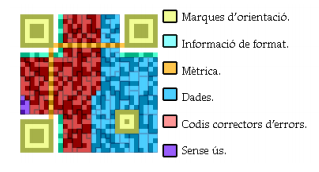
\includegraphics[scale=1]{Fotos/EstructuraCodiQR.png}
    \end{center}
    \caption{Estructura dels Codis QR}
    \label{fig:compiler_phases}
  \end{figure}

\subsubsection{Generar Codi QR}

En aquest projecte l'encarregat de fer el codi QR i mostrar-lo als usuaris és el \emph{front-end} de l'aplicació. Encara que
l'encarregat de generar el text és el servidor. \autoref{chap:back-end}

\subsubsection{Lectura Codi QR}


En aquest projecte l'encarregat de fer la lectura del QR és la Raspberry Pi actuant com a barrera fent servir una càmera.
\autoref{chap:raspberryPi}

\section{Altres aplicacions}
De les diferents alternatives que s'ha explicat en el capítol anterior \autoref{sec:alternatives}
existeixen diferents aplicacions que hi ha al mercat que solucionen el problema real
són les següents:

\begin{enumerate}
    \item \texttt{telpark}: Una aplicació amb la possibilitat de reservar una plaça de pàrquing posar el pàrquing on es vol
    aparcar, posar la durada amb possibilitat d'augmentar el temps, el vehicle i la forma de pagament.
    Possibilitat de pagar el parquímetre \autocite{telpark}.
    \item \texttt{Parkingdoor}: Aquesta aplicació és útil en garatges privats, quan es vol estalviar el comandament
    per pujar la porta del garatge. S'ha d'insta\l.lar un dispositiu junt la porta i el dispositiu mòbil que actua
    com a comandament. Com s'ha explicat en l'apartat de \autoref{sssec:alternatives}.
    Més informació a \autocite{parkingdoor}.
    \item \texttt{El Parking}: Aquesta aplicació dóna la possibilitat de fer pagaments a través de l'aplicació.
    Fer reserves amb la possibilitat de cance\l.lació. Més informació a \autocite{el_parking}.
\end{enumerate}

Totes aquestes aplicacions tenen la característica de funcionar amb diferents pàrquings a la vegada.
L'aplicació d'aquest projecte es basa en la creació de la gestió d'un pàrquing privat, d'una institució o la
possibilitat de ser un pàrquing públic. On la configuració d'aquests és única i personal, és a dir, l'aplicació és feta a mida per
a cada un dels pàrquings. A més a més, amb la funcionalitat d'usar els codis QR per les entrades i sortides del pàrquing.